\documentclass{../../../kin_math}

\header{Elijah Kin}{Homework 8}{AMSC660}
\headrule

\begin{document}

\begin{questions}
  \question Prove that the conjugate gradient algorithm, the preliminary version (Algorithm 5.1, page 108 in [NW]), is equivalent to Algorithm 5.2 (CG) (page 112 in [NW]), i.e., that
  \begin{equation}
    \alpha_k = \frac{r_k^\top r_k}{p_k^\top A p_k} \text{ and } \beta_{k + 1} = \frac{r_{k + 1}^\top r_{k + 1}}{r_k^\top r_k}.
  \end{equation}
  \begin{solution}
    Recall from Algorithm 5.1, that we defined
    \begin{equation*}
      \alpha_k \coloneqq - \frac{r_k^\top p_k}{p_k^\top A p_k} \text{ and } \beta_{k + 1} \coloneqq \frac{r_{k + 1}^\top A p_k}{p_k^\top A p_k}.
    \end{equation*}
    We first show the result for $\alpha_k$; expanding the definition of $p_k$,
    \begin{equation*}
      \alpha_k \coloneqq - \frac{r_k^\top p_k}{p_k^\top A p_k} = - \frac{r_k^\top (-r_k + \beta_k p_{k - 1})}{p_k^\top A p_k} = \frac{r_k^\top r_k - \beta_k r_k^\top p_{k - 1}}{p_k^\top A p_k}
    \end{equation*}
    but recall that $r_k^\top p_i = 0$ for $i = 0, 1, \dots, k - 1$, and hence $r_k^\top p_{k - 1} = 0$. Therefore,
    \begin{equation*}
      \alpha_k = \frac{r_k^\top r_k - \beta_k r_k^\top p_{k - 1}}{p_k^\top A p_k} = \frac{r_k^\top r_k}{p_k^\top A p_k}
    \end{equation*}
    as desired; note that the right-hand side is the definition of $\alpha_k$ in Algorithm 5.2. Now for $\beta_{k + 1}$, first multiplying by $\alpha_k / \alpha_k$ and using the above result for the $\alpha_k$ in the denominator,
    \begin{equation*}
      \beta_{k + 1} \coloneqq \frac{r_{k + 1}^\top A p_k}{p_k^\top A p_k} = \frac{r_{k + 1}^\top \alpha_k A p_k}{p_k^\top \alpha_k A p_k} = \frac{r_{k + 1}^\top \alpha_k A p_k}{\alpha_k p_k^\top A p_k} = \frac{r_{k + 1}^\top \alpha_k A p_k}{r_k^\top r_k}.
    \end{equation*}
    Finally, recalling the fact that $r_{k + 1} = r_k + \alpha_k A p_k$ and hence $\alpha_k A p_k = r_{k + 1} - r_k$, and also that $r_{k + 1}^\top r_k = 0$, we obtain the desired result
    \begin{equation*}
      \beta_{k + 1} = \frac{r_{k + 1}^\top \alpha_k A p_k}{r_k^\top r_k} = \frac{r_{k + 1}^\top (r_{k + 1} - r_k)}{r_k^\top r_k} = \frac{r_{k + 1}^\top r_{k + 1} - r_{k + 1}^\top r_k}{r_k^\top r_k} = \frac{r_{k + 1}^\top r_{k + 1}}{r_k^\top r_k}
    \end{equation*}
    which is the definition of $\beta_{k + 1}$ in Algorithm 5.2. Hence, the preliminary and practical versions of the conjugate gradient descent algorithm are equivalent.
  \end{solution}

  \question Let $A$ be an $n \times n$ matrix. A subspace spanned by the columns of an $n \times k$ matrix $B$ is an invariant subspace of $A$ if $A$ maps it into itself, i.e., if $AB \subset \textsf{span}(B)$. This means that there is a $k \times k$ matrix $C$ such that $AB = BC$. Prove that if a vector $r \in \mathbb{R}^n$ lies in the $k$-dimensional subspace spanned by the columns of $B$, i.e., if $r = By$ for some $y \in \mathbb{R}^k$ ($r$ is a linear combination of columns of $B$ with coefficients $y_1, \dots, y_k$) then the Krylov subspaces generated by $r$ stop expanding at degree $k - 1$,
  i.e,
  \begin{equation}
    \textsf{span}\{r, Ar, \dots, A^p r\} = \textsf{span}\{r, Ar, \dots, A^{k - 1} r\} \quad \forall p \geq k.
  \end{equation}
  \begin{solution}
    We proceed by induction on $p$. As a base case, consider $p = k$. In particular, we want to show that
    \begin{equation*}
      \textsf{span}\{r, Ar, \dots, A^{k - 1} r, A^k r\} = \textsf{span}\{r, Ar, \dots, A^{k - 1} r\}
    \end{equation*}
    which is true if and only if $A^k r \in \textsf{span}\{r, Ar, \dots, A^{k - 1} r\}$. But since $r = By$ and $AB = BC$, this is equivalent to asking whether
    \begin{equation*}
     BC^k y = A^k B y = A^k r \in \textsf{span}\{r, Ar, \dots, A^{k - 1} r\} = \textsf{span}\{By, BCy, \dots, BC^{k - 1} y\}.
    \end{equation*}
    In particular, this means we want to know whether there exist constants $d_0, d_1, \dots, d_{k - 1}$ such that
    \begin{equation*}
      BC^k y = d_0 By + d_1 BC y + \dots + d_{k - 1} B C^{k - 1} y = B(d_0 I + d_1 C + \dots + d_{k - 1} C^{k - 1})y.
    \end{equation*}
    Hence, the claim is true for the base case if we can write
    \begin{equation*}
      C^k = d_0 I + d_1 C + \dots + d_{k - 1} C^{k - 1}
    \end{equation*}
    and indeed we can. The Cayley-Hamilton theorem states that $C$ is a root of its own characteristic polynomial. Hence, negating the coefficient of the characteristic polynomial allows us to write $C^k$ as a linear combination of $I, C, \dots, C^{k - 1}$. Hence, we have that
    \begin{equation*}
      A^k r = BC^k y \in \textsf{span}\{By, BCy, \dots, BC^{k - 1} y\} = \textsf{span}\{r, Ar, \dots, A^{k - 1} r\}
    \end{equation*}
    so indeed the claim holds when $p = k$.

    Now as the inductive hypothesis suppose the claim holds for some $p \geq k$ and consider the case of $p + 1$. We claim that
    \begin{equation*}
      \textsf{span}\{r, Ar, \dots, A^p r, A^{p + 1} r\} = \textsf{span}\{r, Ar, \dots, A^p r\}
    \end{equation*}
    or equivalently, that $A^{p + 1} r \in \textsf{span}\{r, Ar, \dots, A^p r\}$. Now observe that $A^{p + 1} r = A A^p r$, and by the inductive hypothesis, $A^p r \in \textsf{span}\{r, Ar, \dots, A^p r\} = \textsf{span}\{r, Ar, \dots, A^{k - 1} r\}$, so we can write
    \begin{equation*}
      A^{p + 1} r = A A^p r = A (c_0 r + c_1 A r + \dots + c_{k - 1} A^{k - 1} r) = c_0 A r + c_1 A^2 r + \dots + c_{k - 1} A^k r.
    \end{equation*}
    Hence, it follows that $A^{p + 1} r \in \textsf{span}\{r, Ar, \dots, A^k r\} = \textsf{span}\{r, Ar, \dots, A^{k - 1} r\}$, and so
    \begin{equation*}
      \textsf{span}\{r, Ar, \dots, A^p r, A^{p + 1} r\} = \textsf{span}\{r, Ar, \dots, A^p r\} = \textsf{span}\{r, Ar, \dots, A^{k - 1} r\},
    \end{equation*}
    so the claim holds for $p + 1$. By the principle of induction, the claim holds for all $p \geq k$.
  \end{solution}

  \question Prove Theorem 5.5 from [NW], page 115. Here are the steps that you need to work out.
  \begin{enumerate}
    \item Construct a polynomial $Q(\lambda)$ of degree $k + 1$ with roots $\lambda_n, \lambda_{n - 1}, \dots, \lambda_{n - k + 1}$, and $\frac{1}{2}(\lambda_1 + \lambda_{n - k})$ such that $Q(0) = 1$.
    \begin{solution}
      In order to have $\lambda_n, \lambda_{n - 1}, \dots, \lambda_{n - k + 1}$ as roots of $Q$, we will base $Q$ on
      \begin{equation*}
        (\lambda_n - \lambda)(\lambda_{n - 1} - \lambda) \dots (\lambda_{n - k + 1} - \lambda) = \prod_{j = n - k + 1}^n (\lambda_{j} - \lambda).
      \end{equation*}
      Further, since we also want $\frac{1}{2}(\lambda_1 + \lambda_{n - k})$ as a root, we multiply the above by a factor of $\left(\frac{1}{2}(\lambda_1 + \lambda_{n - k}) - \lambda \right)$ to obtain
      \begin{equation*}
        \left(\frac{1}{2}(\lambda_1 + \lambda_{n - k}) - \lambda \right) \prod_{j = n - k + 1}^n (\lambda_j - \lambda).
      \end{equation*}
      It remains to scale the above by a constant factor to ensure $Q(0) = 1$. Substituting $\lambda = 0$ into the above, we find
      \begin{equation*}
        \frac{1}{2}(\lambda_1 + \lambda_{n - k}) \prod_{j = n - k + 1}^n \lambda_j
      \end{equation*}
      and hence we define
      \begin{multline*}
        Q(\lambda) \coloneqq \frac{\left(\frac{1}{2}(\lambda_1 + \lambda_{n - k}) - \lambda \right) \prod_{j = n - k + 1}^{n} (\lambda_j - \lambda)}{\frac{1}{2}(\lambda_1 + \lambda_{n - k}) \prod_{j = n - k + 1}^n \lambda_j} \\
        = \frac{\frac{1}{2}(\lambda_1 + \lambda_{n - k}) - \lambda}{\frac{1}{2}(\lambda_1 + \lambda_{n - k})} \prod_{j = n - k + 1}^n \left(1 - \frac{\lambda}{\lambda_j}\right).
      \end{multline*}
    \end{solution}
    \item Argue that $P(\lambda)$ defined as
    \begin{equation}
      P(\lambda) = \frac{Q(\lambda) - 1}{\lambda}
    \end{equation}
    is a polynomial, not a rational function, by referring to the theorem about factoring polynomials. Cite that theorem.
    \begin{solution}
      Recall that we constructed $Q(\lambda)$ such that $Q(0) = 1$, so the polynomial $Q(\lambda) - 1$ has a root at $0$. In particular, by the factor theorem this means that we can write
      \begin{equation*}
        Q(\lambda) - 1 = (\lambda - 0) P(\lambda) = \lambda P(\lambda)
      \end{equation*}
      for some polynomial $P(\lambda)$. Hence,
      \begin{equation*}
        P(\lambda) = \frac{Q(\lambda) - 1}{\lambda}
      \end{equation*}
      is indeed a polynomial.
    \end{solution}
    \item Use the ansatz
    \begin{equation}
      \lVert x_{k + 1} - x^* \rVert_A^2 \leq \min_{P \in \mathcal{P}_k} \max_{1 \leq i \leq n} [1 + \lambda_i P(\lambda_i)]^2 \lVert x_0 - x^* \rVert_A^2.
    \end{equation}
    Argue that
    \begin{equation}
      \lVert x_{k + 1} - x^* \rVert_A^2 \leq \max_{1 \leq i \leq n} Q^2(\lambda_i) \lVert x_0 - x^* \rVert_A^2.
    \end{equation}
    \begin{solution}
      Taking as an ansatz,
      \begin{equation*}
        \lVert x_{k + 1} - x^* \rVert_A^2 \leq \min_{P_k \in \mathcal{P}_k} \max_{1 \leq i \leq n} [1 + \lambda_i P_k(\lambda_i)]^2 \lVert x_0 - x^* \rVert_A^2
      \end{equation*}
      then in particular it must be that
      \begin{equation*}
        \lVert x_{k + 1} - x^* \rVert_A^2 \leq \max_{1 \leq i \leq n} [1 + \lambda_i P(\lambda_i)]^2 \lVert x_0 - x^* \rVert_A^2
      \end{equation*}
      since $P$ is a polynomial of degree $k$ by item (b), since $Q$ is a polynomial of degree $k + 1$. Further, by definition
      \begin{equation*}
        P(\lambda_i) = \frac{Q(\lambda_i) - 1}{\lambda_i}
      \end{equation*}
      and hence $1 + \lambda_i P(\lambda_i) = Q(\lambda_i)$, meaning
      \begin{equation*}
        \lVert x_{k + 1} - x^* \rVert_A^2 \leq \max_{1 \leq i \leq n} [1 + \lambda_i P(\lambda_i)]^2 \lVert x_0 - x^* \rVert_A^2 = \max_{1 \leq i \leq n} [Q(\lambda_i)]^2 \lVert x_0 - x^* \rVert_A^2
      \end{equation*}
      as desired.
    \end{solution}
    \item Show that
    \begin{equation}
      \lVert x_{k + 1} - x^* \rVert_A^2 \leq \max_{\lambda \in [\lambda_1, \lambda_{n - k}]} \left| \frac{\lambda - \frac{1}{2}(\lambda_1 + \lambda_{n - k})}{\frac{1}{2}(\lambda_1 + \lambda_{n - k})} \right|^2 \lVert x_0 - x^* \rVert_A^2.
    \end{equation}
    \begin{solution}
      From item (c), we know that
      \begin{equation*}
        \lVert x_{k + 1} - x^* \rVert_A^2 \leq \max_{1 \leq i \leq n} Q^2(\lambda_i) \lVert x_0 - x^* \rVert_A^2
      \end{equation*}
      hence it suffices to show that
      \begin{equation*}
        \max_{1 \leq i \leq n} Q^2(\lambda_i) \leq \max_{\lambda \in [\lambda_1, \lambda_{n - k}]} \left| \frac{\lambda - \frac{1}{2}(\lambda_1 + \lambda_{n - k})}{\frac{1}{2}(\lambda_1 + \lambda_{n - k})} \right|^2.
      \end{equation*}
      Toward this end, recall that by construction, $Q(\lambda_i) = 0$ for $n - k + 1 \leq i \leq n$. Hence,
      \begin{equation*}
        \max_{1 \leq i \leq n} Q^2(\lambda_i) = \max_{1 \leq i \leq n - k} Q^2(\lambda_i).
      \end{equation*}
      Further, it is certainly true that
      \begin{equation*}
        \max_{1 \leq i \leq n - k} Q^2(\lambda_i) \leq \max_{\lambda \in [\lambda_1, \lambda_{n - k}]} Q^2(\lambda),
      \end{equation*}
      hence we need only show that
      \begin{equation*}
        \max_{\lambda \in [\lambda_1, \lambda_{n - k}]} Q^2(\lambda) \leq \max_{\lambda \in [\lambda_1, \lambda_{n - k}]} \left| \frac{\lambda - \frac{1}{2}(\lambda_1 + \lambda_{n - k})}{\frac{1}{2}(\lambda_1 + \lambda_{n - k})} \right|^2.
      \end{equation*}
      Recalling our definition of $Q$, we have that
      \begin{multline*}
        Q^2(\lambda) = \left(\frac{\frac{1}{2}(\lambda_1 + \lambda_{n - k}) - \lambda}{\frac{1}{2}(\lambda_1 + \lambda_{n - k})}\right)^2 \prod_{j = n - k + 1}^n \left(1 - \frac{\lambda}{\lambda_j}\right)^2 \\
        = \left|\frac{\lambda - \frac{1}{2}(\lambda_1 + \lambda_{n - k})}{\frac{1}{2}(\lambda_1 + \lambda_{n - k})}\right|^2 \prod_{j = n - k + 1}^n \left(1 - \frac{\lambda}{\lambda_j}\right)^2
      \end{multline*}
      and so the result follows provided for all $\lambda \in [\lambda_1, \lambda_{n - k}]$,
      \begin{equation*}
        \prod_{j = n - k + 1}^n \left(1 - \frac{\lambda}{\lambda_j}\right)^2 \leq 1.
      \end{equation*}
      To see that this inequality is true, take $j \in \{n - k + 1, \dots, n\}$ and $\lambda \in [\lambda_1, \lambda_{n - k}]$. Then
      \begin{equation*}
        \frac{\lambda}{\lambda_j} \leq \frac{\lambda}{\lambda_{n - k + 1}} \leq \frac{\lambda_{n - k}}{\lambda_{n - k + 1}} < 1
      \end{equation*}
      and also $\frac{\lambda}{\lambda_j} > 0$ since $A$ is SPD; hence $\left(1 - \frac{\lambda}{\lambda_j}\right)^2 \leq 1$, so $\prod_{j = n - k + 1}^n \left(1 - \frac{\lambda}{\lambda_j}\right)^2 \leq 1$. Therefore,
      \begin{multline*}
        \max_{\lambda \in [\lambda_1, \lambda_{n - k}]} Q^2(\lambda) = \max_{\lambda \in [\lambda_1, \lambda_{n - k}]} \left|\frac{\lambda - \frac{1}{2}(\lambda_1 + \lambda_{n - k})}{\frac{1}{2}(\lambda_1 + \lambda_{n - k})}\right|^2 \prod_{j = n - k + 1}^n \left(1 - \frac{\lambda}{\lambda_j}\right)^2 \\
        \leq \max_{\lambda \in [\lambda_1, \lambda_{n - k}]} \left| \frac{\lambda - \frac{1}{2}(\lambda_1 + \lambda_{n - k})}{\frac{1}{2}(\lambda_1 + \lambda_{n - k})} \right|^2
      \end{multline*}
      and so we obtain the desired result by applying item (c).
    \end{solution}
    \item Find the maximum of the function in the right-hand side of the last equation in the interval $[\lambda_1, \lambda_{n - k}]$.
    \begin{solution}
      The maximum is attained either at an endpoint of the interval $[\lambda_1, \lambda_{n - k}]$, or at a critical point. Differentiating, we find
      \begin{equation*}
        \frac{d}{d\lambda} \left| \frac{\lambda - \frac{1}{2}(\lambda_1 + \lambda_{n - k})}{\frac{1}{2}(\lambda_1 + \lambda_{n - k})} \right|^2 = \frac{d}{d\lambda} \left( \frac{\lambda - \frac{1}{2}(\lambda_1 + \lambda_{n - k})}{\frac{1}{2}(\lambda_1 + \lambda_{n - k})} \right)^2 = 2 \left( \frac{\lambda - \frac{1}{2}(\lambda_1 + \lambda_{n - k})}{\frac{1}{2}(\lambda_1 + \lambda_{n - k})} \right).
      \end{equation*}
      We see that the above is equal to 0 if and only if $\lambda = \frac{1}{2}(\lambda_1 + \lambda_{n - k})$, giving us a third candidate maximizer. We will now evaluate the right-hand side for each of $\lambda_1$, $\lambda_{n - k}$, and $\frac{1}{2}(\lambda_1 + \lambda_{n - k})$.

      At $\lambda_1$, we find
      \begin{equation*}
        \left| \frac{\lambda_1 - \frac{1}{2}(\lambda_1 + \lambda_{n - k})}{\frac{1}{2}(\lambda_1 + \lambda_{n - k})} \right|^2 = \left| \frac{\frac{1}{2}(\lambda_1 - \lambda_{n - k})}{\frac{1}{2}(\lambda_1 + \lambda_{n - k})} \right|^2 = \left| \frac{\lambda_1 - \lambda_{n - k}}{\lambda_1 + \lambda_{n - k}} \right|^2
      \end{equation*}
      which we see is non-negative. The situation is similar for $\lambda_{n - k}$, where
      \begin{equation*}
        \left| \frac{\lambda_{n - k} - \frac{1}{2}(\lambda_1 + \lambda_{n - k})}{\frac{1}{2}(\lambda_1 + \lambda_{n - k})} \right|^2 = \left| \frac{-\frac{1}{2}(\lambda_1 - \lambda_{n - k})}{\frac{1}{2}(\lambda_1 + \lambda_{n - k})} \right|^2 = \left| \frac{\lambda_1 - \lambda_{n - k}}{\lambda_1 + \lambda_{n - k}} \right|^2
      \end{equation*}
      and so $\lambda_1$ and $\lambda_{n - k}$ achieve the same value on the right-hand side. It remains to check $\frac{1}{2}(\lambda_1 + \lambda_{n - k})$.
      \begin{equation*}
        \left| \frac{\frac{1}{2}(\lambda_1 + \lambda_{n - k}) - \frac{1}{2}(\lambda_1 + \lambda_{n - k})}{\frac{1}{2}(\lambda_1 + \lambda_{n - k})} \right|^2 = 0,
      \end{equation*}
      and so the maximum is attained at $\lambda_1$ and $\lambda_{n - k}$, meaning
      \begin{equation*}
        \max_{\lambda \in [\lambda_1, \lambda_{n - k}]} \left| \frac{\lambda - \frac{1}{2}(\lambda_1 + \lambda_{n - k})}{\frac{1}{2}(\lambda_1 + \lambda_{n - k})} \right|^2 = \left| \frac{\lambda_1 - \lambda_{n - k}}{\lambda_1 + \lambda_{n - k}} \right|^2.
      \end{equation*}
    \end{solution}
    \item Finish the proof of the theorem.
    \begin{solution}
      From item (d) we have that
      \begin{equation*}
        \lVert x_{k + 1} - x^* \rVert_A^2 \leq \max_{\lambda \in [\lambda_1, \lambda_{n - k}]} \left| \frac{\lambda - \frac{1}{2}(\lambda_1 + \lambda_{n - k})}{\frac{1}{2}(\lambda_1 + \lambda_{n - k})} \right|^2 \lVert x_0 - x^* \rVert_A^2
      \end{equation*}
      and from item (e) we have
      \begin{equation*}
        \max_{\lambda \in [\lambda_1, \lambda_{n - k}]} \left| \frac{\lambda - \frac{1}{2}(\lambda_1 + \lambda_{n - k})}{\frac{1}{2}(\lambda_1 + \lambda_{n - k})} \right|^2 = \left| \frac{\lambda_1 - \lambda_{n - k}}{\lambda_1 + \lambda_{n - k}} \right|^2.
      \end{equation*}
      Taking these facts together we obtain
      \begin{equation*}
        \lVert x_{k + 1} - x^* \rVert_A^2 \leq \left| \frac{\lambda_1 - \lambda_{n - k}}{\lambda_1 + \lambda_{n - k}} \right|^2 \lVert x_0 - x^* \rVert_A^2
      \end{equation*}
      which is the claim of Theorem 5.5.
    \end{solution}
  \end{enumerate}

  \question \emph{The coding for this problem can be done in Matlab or Python. If you choose Python, you can export the matrix $L_\textsf{symm}$ and the vector $b_\textsf{symm}$ to Python and do the rest of the work in Python.} The goal of this problem is to practice the \emph{conjugate gradient algorithm (CG) with and without preconditioning} on a meaningful problem. An explanation for its setup is a bit long, but it is a typical case that a lot of effort is spent on problem setup. I have done the setup for you. Your job will be just to code the CG algorithms.
  \begin{figure}
    \centering
    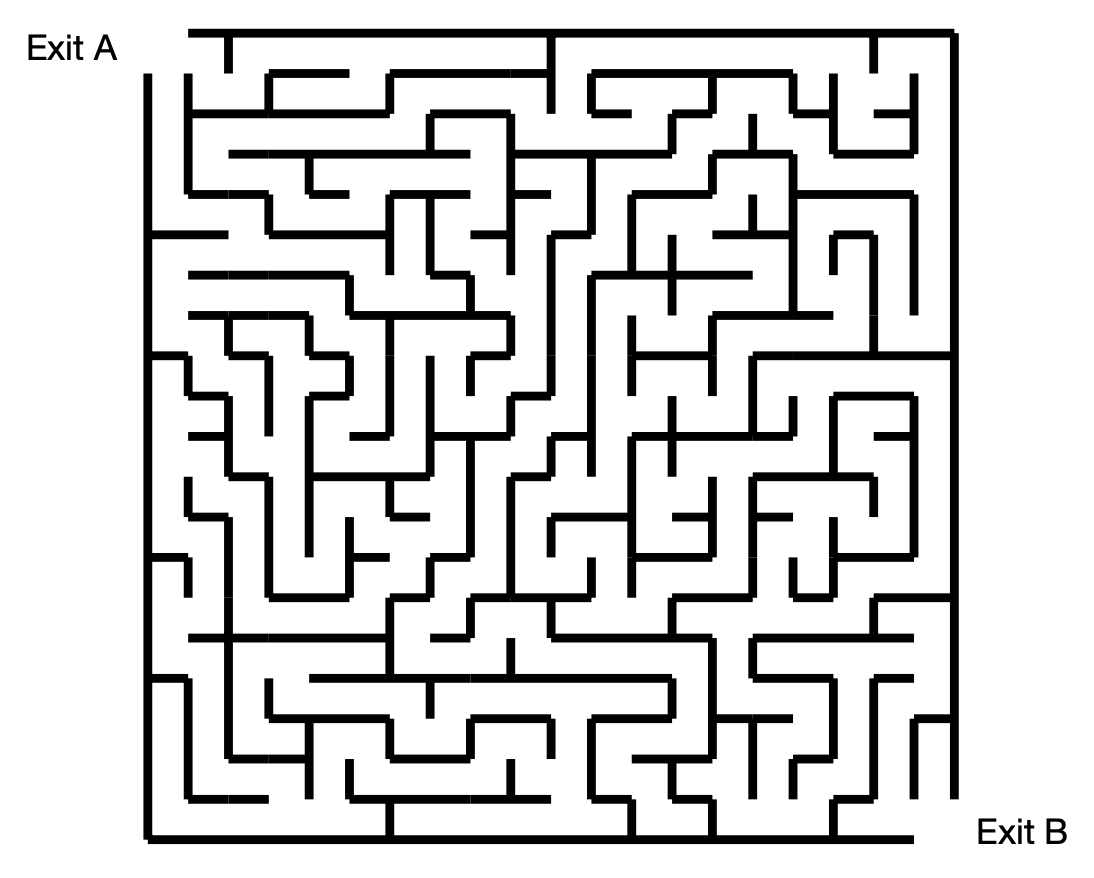
\includegraphics[scale=0.5]{maze.png}
    \caption{A maze with two exits.}
  \end{figure}
  Consider a maze with two exists, A, and B, shown in Fig. 1 taken from \href{https://www.researchgate.net/publication/23464509_Transition-Path_Theory_and_Path-Finding_Algorithms_for_the_Study_of_Rare_Events}{this paper} by W. Ee and E. Vanden-Eijnden. This maze consists of a $20 \times 20$ array of cells, $N = 400$ cells in total. We will number the calls from 1 to 400 column-wise, i.e., the first column contains cells with indices from 1 to 20, the second one from 21 to 40, and so on. Exit A is at cell 1 while Exit B is at cell 400.

  Let $A$ be the adjacency matrix for this maze. $A$ is $400 \times 400$, $A_{ij} = 1$ if cells $i$ and $j$ are adjacent and there is no wall between them, and $A_{ij} = 0$ otherwise. A random walker makes a step from a cell to any adjacent cell not separated by a wall with equal probability. The stochastic matrix (the other names for it are the transition matrix and the Markov matrix) for this random walk can be found as $P = R^{-1} A$ where $R$ is a diagonal matrix with row sums of $A$ along its diagonal. Row rums of $P$ are all equal to 1, and $P_{ij}$ is the probability that the random walker located at cell $i$ will next move to cell $j$.

  Our goal is to compute the \emph{committor} $x \in \mathbb{R}^N$ for this random walk, i.e., the vector of probabilities whose component $x_i$ is the probability that the walker located at cell $i$ will first arrive at Exit B rather than Exit A. This vector of probabilities satisfies:
  \begin{equation}
    \label{eq:probs}
    x_1 = 0, \quad x_N = 1, \quad x_i = \sum_{j = 1}^N P_{ij} x_j, \quad 2 \leq i \leq N - 1.
  \end{equation}
  Equation (\ref{eq:probs}) is obtained from the following reasoning. The probability of exiting via B rather than A from cell $i$ is equal to the sum of products of probabilities to a cell $j$ from $i$ and exit from $j$ via B rather than A. The sum is over all other cells $j$. Equation (\ref{eq:probs}) can be written in the matrix form as follows. We denote $P - I$ by $L$. Then
  \begin{equation}
    L_{2:(N - 1), 2:(N - 1)} x_{2:(N - 1)} = b_{2:(N - 1)},
  \end{equation}
  where $b$ is obtained by $b = -Le_N$, where $e_N$ is the vector with entries $1, \dots, N - 1$ equal to zero and entry $N$ equal to 1. You can check this, or just believe me. Recall that $L = R^{-1} A - I$. It is not a symmetric matrix, but it can be symmetrized as follows. We will mark with tilde all submatrices $(2 : (N - 1), 2 : (N - 1))$ and all subvectors with indices in $2 : (N - 1)$. Then we symmetrize $\tilde{L}$ using the fact that the adjacency matrix $A$ is symmetric, $\tilde{L} = \tilde{R}^{-1} \tilde{A} - \tilde{I}$, and multiplication by $\tilde{R}^{\pm 1 / 2}$.
  \begin{align}
    \tilde{L} \tilde{x} &= \tilde{b}, \quad \text{the linear system we need to solve;} \\
    (\tilde{R}^{-1} \tilde{A} - \tilde{I}) \tilde{x} &= \tilde{b}, \quad \text{recall what is $\tilde{L}$;} \\
    \tilde{R}^{1/2} (\tilde{R}^{-1} \tilde{A} - \tilde{I}) \tilde{R}^{-1/2} \tilde{R}^{1/ 2} \tilde{x} &= \tilde{R}^{1 / 2} \tilde{b}, \quad \text{multiply by $\tilde{R}^{1/2}$, insert $\tilde{R}^{-1/2} \tilde{R}^{1/ 2}$;} \\
    (\tilde{R}^{-1/2} \tilde{A} \tilde{R}^{-1/2} - \tilde{I}) \tilde{R}^{1/ 2} \tilde{x} &= \tilde{R}^{1 / 2} \tilde{b}, \quad \text{do some algebra.}
  \end{align}
  The matrix $\tilde{R}^{-1/2} \tilde{A} \tilde{R}^{-1/2} - \tilde{I}$ is symmetric. $\tilde{R}^{1/2} \tilde{x} \eqqcolon y$ is a new vector of unknowns. $\tilde{R}^{1/2} \tilde{b} \eqqcolon b_\textsf{symm}$ is the new right-hand side. It is possible to check (just believe me), that the matrix $-L_\textsf{symm}$ is symmetric positive definite.

  Thus, here is the linear system with a symmetric positive definite matrix:
  \begin{equation}
    \label{eq:boxed}
    \boxed{-L_\textsf{symm} y = -b_\textsf{symm}, \quad x_{2:(N - 1)} = \tilde{R}^{-1/2}y.}
  \end{equation}
  The Matlab code \texttt{random\_walk\_in\_maze.m} visualizes the maze, sets up this linear system, solves it using the built-in solver ``\textbackslash'', visualizes the solution, and plots the eigenvalues of $-L_\textsf{symm}$. Task. Modify the code to solve Eq. (\ref{eq:boxed}) using the conjugate gradient algorithm without and with preconditioning (Algorithms 5.2 and 5.3) in [NW]. Use the incomplete Cholesky preconditioner. The corresponding Matlab command is
  \begin{verbatim}
    ichol_fac = ichol(sparse(A));
    M = ichol_fac * ichol_fac';\end{verbatim}
Stop iterations when the residual will have a norm less than $10^{-12}$. Plot the norm of the residuals after each iteration for the CG algorithm with and without preconditioning in the same figure. Use the logarithmic scale along the y-axis. Visualize the computed solution. Link you code to the pdf file with the homework.

  \emph{The coding for this problem can be done in Matlab or Python. If you choose Python, you can export the matrix $L_\textsf{symm}$ and the vector $b_\textsf{symm}$ to Python and do the rest of the work in Python.}
  \begin{solution}
    We plot the convergence of the two algorithms below via the code \href{https://github.com/elijahkin/school/blob/main/umd/amsc660/hw8/hw8.ipynb}{here}
    \begin{figure}
      \centering
      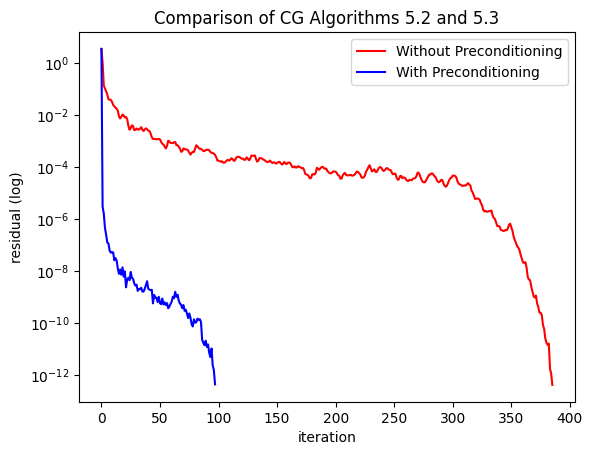
\includegraphics[scale=0.7]{cg.png}
    \end{figure}
    We see that the algorithm without conditioning takes about 380 iterations for the residual to not exceed $10^{-12}$, while with conditioning, it takes only 100 iterations.
  \end{solution}
\end{questions}

\end{document}
